\documentclass[a4paper,11pt]{article}

\usepackage{cmap}		
%\usepackage[utf8]{inputenc}			
\usepackage[brazil]{babel}
\usepackage{framed}
\usepackage{hyperref}
\usepackage{amsmath}
\usepackage{graphicx}
\usepackage[colorinlistoftodos]{todonotes}
\usepackage{wrapfig}
\usepackage{lipsum}
\usepackage{listings}
\usepackage{color}
\usepackage{indentfirst}
\usepackage{times}
\usepackage{textcomp}
\usepackage{pgfgantt}
\usepackage{lipsum}

% set document font, font sizes, margin dimensions and spacing
\usepackage{fontspec}
\setmainfont{Arial}
\usepackage[top=15mm,bottom=25mm,left=20mm,right=20mm]{geometry}
\usepackage{setspace}\onehalfspacing
\usepackage{titlesec}
\titleformat*{\section}{\Large\bfseries}
\titleformat*{\subsection}{\Large\bfseries}
\titleformat*{\subsubsection}{\Large\bfseries}
\titleformat*{\paragraph}{\Large\bfseries}
\titleformat*{\subparagraph}{\Large\bfseries}
\setlength{\parskip}{0.6em}

\newif\ifblackandwhite
\blackandwhitetrue

\usepackage{etoolbox}
\usepackage{longtable}%
\AtBeginEnvironment{longtable}{%
  \addfontfeature{RawFeature=+tnum;-onum}%  <--- requires LuaTeX
}

\usepackage{pdflscape}
%\usepackage[svgnames]{xcolor}
 \usepackage{colortbl}%
   \newcommand{\myrowcolour}{\rowcolor[gray]{0.925}}
\usepackage{booktabs}

\ifblackandwhite
  \newcommand{\cheading}[2]{\textbf{#1\hfill #2}}
  \newcommand{\highest}[1]{\textbf{#1}}% == highest score for question
\else
  \newcommand{\cheading}[2]{\textcolor{Maroon}{\textbf{#1\hfill #2}}}
  \newcommand{\highest}[1]{\textcolor{Maroon}{\textbf{#1}}}%
\fi

\definecolor{mygray}{rgb}{0.4,0.4,0.4}
\definecolor{mygreen}{rgb}{0,0.8,0.6}
\definecolor{myorange}{rgb}{1.0,0.4,0}

\lstdefinestyle{customc}{
  belowcaptionskip=1\baselineskip,
  breaklines=true,
  frame=L,
  xleftmargin=\parindent,
  language=C,
  showstringspaces=false,
  basicstyle=\footnotesize\ttfamily,
  keywordstyle=\bfseries\color{green!40!black},
  commentstyle=\itshape\color{purple!40!black},
  identifierstyle=\color{blue},
  stringstyle=\color{orange},
  numbers=left,
  numbersep=12pt,
  numberstyle=\small\color{mygray},
}
\lstset{escapechar=@,style=customc}

\newcommand{\HRule}{\rule{\linewidth}{0.5mm}}

%Definindo um comando todoin que aceita quebra de linha e fórmulas
\newcommand\todoin[2][]{\todo[inline, caption={2do}, #1]{
\begin{minipage}{\textwidth-4pt}#2\end{minipage}}}

\newcommand\todogeg[2][]{\todo[inline, caption={#2}, color=yellow!100, #1]{
\begin{minipage}{\textwidth-4pt}#2\end{minipage}}}

\newcommand\todovwcm[2][]{\todo[inline, caption={#2}, color=red!100, #1]{
\begin{minipage}{\textwidth-4pt}#2\end{minipage}}}

\begin{document}

\begin{titlepage}
    \begin{center}

        % logo
        
\includegraphics[width=0.15\textwidth]{images/ufsc_logo_sf.png}~
        \\[2cm]

        \textsc{\large <Título do Plano de Trabalho do Aluno>(Aqui escreve MIGMASTATS?)}
        \\[2cm]

        % identificação do relatório
        \HRule \\[0.4cm]
        {\large \bfseries Relatório Final das atividades do Programa Institucional \\
        de Bolsas de Iniciação Científica e Voluntário PIBIC \\
        Edital 2021\\[0.4cm]}
        \HRule
        \\[2cm]

        % identificação do aluno
        \large\textbf{Aluno}\\
        Rodrigo Ferraz Souza\\
        Engenharia de Computação \\
        Programa PIBIC
        \\[1cm]

        % identificação do orientador
        \large\textbf{Orientador}\\
        Antônio Carlos Sobieranski\\
        <Departamento/Unidade Acadêmica> (não sei o que é isso)
        \\[1cm]

        % identificação do projeto de pesquisa
        \large\textbf{Projeto de Pesquisa}\\
        Análise Estatística do Dataset MIGMA (ver depois no doc que eu assinei)\\[1cm]


        \vfill

        % Bottom of the page
        {\large \today}

    \end{center}
\end{titlepage}

\newpage
\begin{abstract}
  no máximo 1 página

\end{abstract}

\newpage
\tableofcontents
\newpage
\section{Introdução}
\label{sec:introducao}

Exemplo de referência para figura

Como visto na Figura~\ref{fig:lifecycle_phase} $\ldots$

\begin{figure}[ht]
    \center
    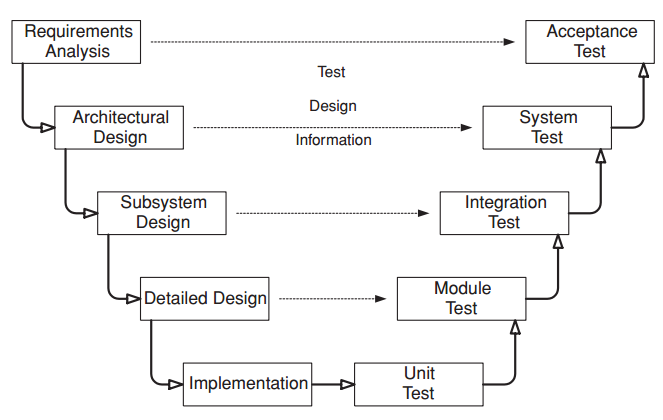
\includegraphics[scale=0.7]{images/lifecycle_phase.png}
    \caption{Testing levels based on software development phase (Sommerville, 2011).}
    \label{fig:lifecycle_phase}
\end{figure}

Exemplo de referência para bibliografia

De acordo com \cite{sommerville2011software} $\ldots$

\section{Objetivos}
\label{sec:objetivos}

Descrever o objetivo geral. Elencar e explicar cada um dos objetivos específicos.

\textbf{Objetivos específicos}

\begin{itemize}
    \item Objetivo específico 1 : 
    \item Objetivo específico 2 : 
\end{itemize}

\section{Metodologia}
\label{sec:metodologia}

Exemplo de referência para seção

Como visto na Seção~\ref{sec:introducao} $\ldots$
\section{Resultados e Discussão}
\label{sec:resultados}
\section{Atividades Relevantes Desenvolvidas pelo Bolsista}
\label{sec:atividades}

Participações em Congressos, Seminários, Cursos etc., trabalhos apresentados e publicados em eventos científicos

\section{Dificuldades Encontradas}
\label{sec:dificuldades}

não relatar dificuldade pessoal, tal como a falta de conhecimento linguístico do bolsista

\section{Cronograma de Execução}
\label{sec:cronograma}

\section{Considerações <Parciais ou Finais>}
\label{sec:consideracoes}
\section{Parecer do Orientador}


\noindent Recife, DD  de MMMMMMM  de 20AA 
\\[1.5cm]
----------------------------------------\\
Assinatura do Orientador\\
\\[1.5cm]
----------------------------------------\\
Assinatura do Aluno
\renewcommand\refname{Referências Bibliográficas}
%\bibliographystyle{abntex2-alf}
\bibliographystyle{IEEEtran}
\bibliography{referencias.bib}
%\listoftodos

\end{document}